\section{Methodology}

\begin{frame}{Chain-of-Thought Prompting}
    Chain-of-Thought prompting~\cite{wei2023chainofthought} -- a series of intermediate reasoning steps -- substantially enhances the capacity of LLMs to engage in complex reasoning, making it a promising approach for code generation.
    \begin{figure}[!htb]
        \centering
        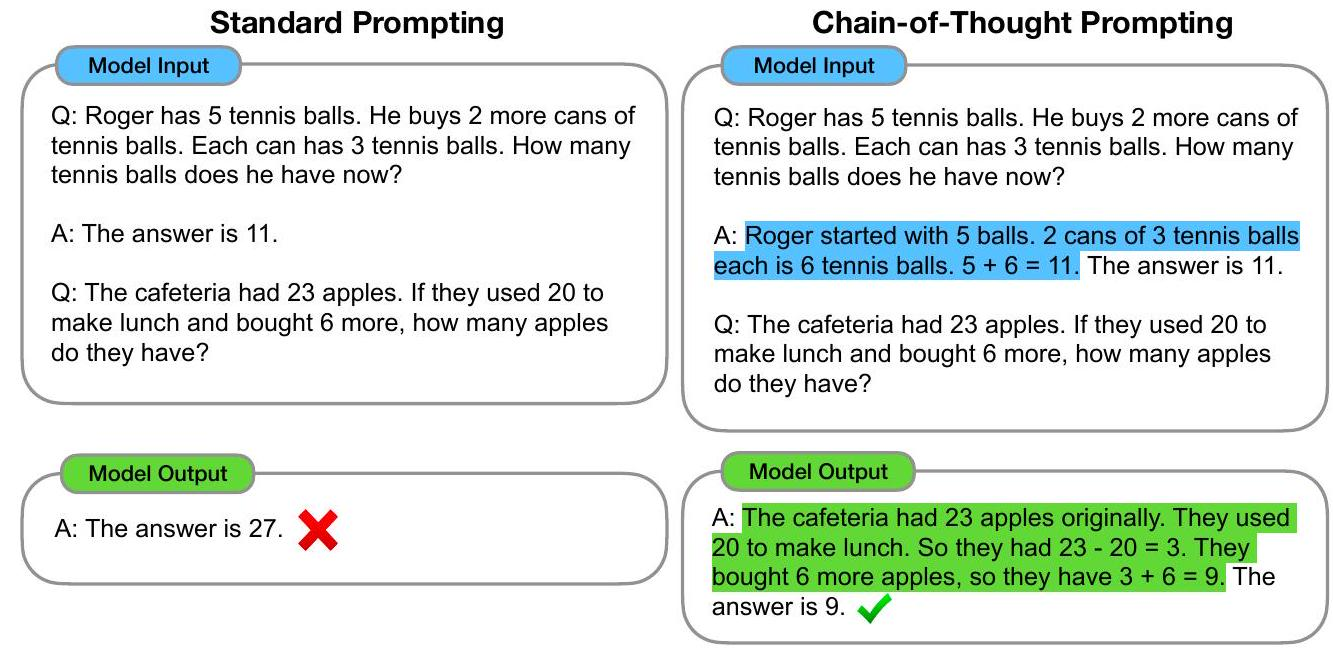
\includegraphics[scale=0.20]{img/cot_prompting}
        \captionsetup{font=small}
        \caption{Chain-of-thought reasoning processes are highlighted.}
    \end{figure}
\end{frame}

\begin{frame}{Modular Code Analysis}
    Modular code analysis, inspired by how developers decompose complex problems into solvable sub-problems, has proven effective for code generation.~\cite{le2023codechain}.
    \begin{figure}[!htb]
        \centering
        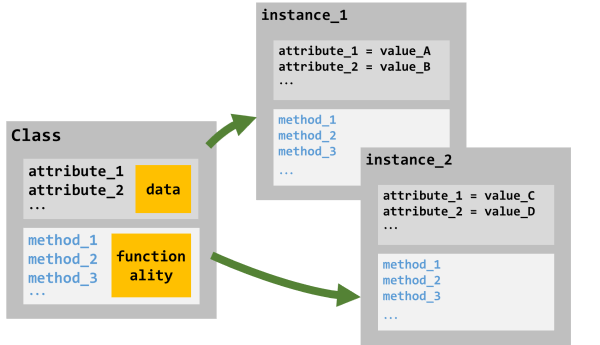
\includegraphics[scale=0.50]{img/class_diagram}
        \captionsetup{font=small}
        \caption{Illustration of code modules.}
    \end{figure}
\end{frame}
